% The title and chapter boundary remain provisional. This chapter is the
% complete working manuscript for the first seminar talk.

\chapter{Why derived manifolds?}\label[chapter]{chap:Why_Derived_Manifolds}

\section{Transverse fiber products}
\label[section]{sec:Transverse_Fiber_Products}

Consider the following two intersections of curves in $\R^2$.

\begin{figure}[ht]
  \centering
  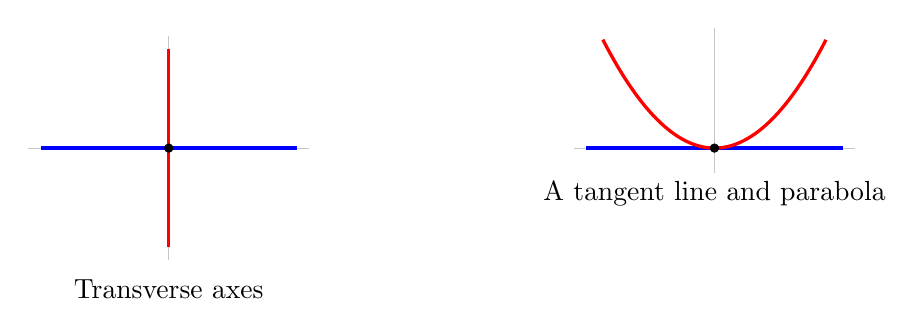
\begin{tikzpicture}[scale=1.05]
    \begin{scope}[xshift=-3.3cm]
      \draw[gray!45] (-1.7,0)--(1.7,0);
      \draw[gray!45] (0,-1.35)--(0,1.35);
      \draw[very thick,blue] (-1.55,0)--(1.55,0);
      \draw[very thick,red] (0,-1.2)--(0,1.2);
      \fill (0,0) circle (1.6pt);
      \node at (0,-1.7) {Transverse axes};
    \end{scope}
    \begin{scope}[xshift=3.3cm]
      \draw[gray!45] (-1.7,0)--(1.7,0);
      \draw[gray!45] (0,-.3)--(0,1.45);
      \draw[very thick,blue] (-1.55,0)--(1.55,0);
      \draw[very thick,red,domain=-1.35:1.35,samples=80]
        plot (\x,{0.72*\x*\x});
      \fill (0,0) circle (1.6pt);
      \node at (0,-.55) {A tangent line and parabola};
    \end{scope}
  \end{tikzpicture}
  \caption{Two intersections with the same underlying set.}
  \label[figure]{fig:Two_Intersections}
\end{figure}

Set-theoretically, the answer is the same in both panels of
\Cref{fig:Two_Intersections}: the intersection consists only of the origin.
Geometrically, the two answers behave very differently. The transverse
intersection is stable locally under sufficiently small perturbations. For the
tangent intersection, replace the parabola by
\[
  y=x^2+\varepsilon.
\]
Its intersection with the $x$-axis consists of two points when
$\varepsilon<0$, one point when $\varepsilon=0$, and no points when
$\varepsilon>0$. The singleton at $\varepsilon=0$ therefore conceals both an
infinitesimal direction and the
obstruction which prevents that direction from extending to an actual family
of solutions.

\begin{question*}
  What geometric object should replace a nontransverse intersection so that it
  remembers the defining equations, agrees with the ordinary intersection in
  the transverse case, and behaves well in families?
\end{question*}

This question is the point of entry to derived manifolds. We will not define
them in this chapter. Instead, we first recall exactly what transversality
provides, then calculate what is lost when it fails, and finally see the same
deformation--obstruction pattern in elliptic moduli problems. The calculations
will give us a short list of requirements that later definitions must satisfy.
The same intersection-theoretic problem is the starting point of Spivak's
construction of derived smooth manifolds
\cite[Sections~1--3]{Spivak_Derived_Smooth_Manifolds}.

Let $f\colon X\to Z$ and $g\colon Y\to Z$ be smooth maps between smooth
manifolds. Their fiber product as sets is
\[
  X\times_ZY
  =\{(x,y)\in X\times Y\mid f(x)=g(y)\}.
\]
Without an additional hypothesis, this subset of $X\times Y$ need not be a
smooth manifold of the expected dimension. Transversality is the hypothesis
which rules out this defect.

\begin{definition}[Transverse maps]\label[definition]{def:Transverse_Maps}
  Let $f\colon X\to Z$ and $g\colon Y\to Z$ be smooth maps. For
  $(x,y)\in X\times_ZY$, with common image $z=f(x)=g(y)$, define the
  \emph{linearized matching map}
  \[
    \delta_{x,y}
    =D_xf-D_yg
    \colon T_xX\oplus T_yY\longrightarrow T_zZ.
  \]
  We say that $f$ and $g$ are \emph{transverse} if $\delta_{x,y}$ is
  surjective for every $(x,y)\in X\times_ZY$.
\end{definition}

Equivalently, $f$ and $g$ are transverse if
\[
  \operatorname{im}(D_xf)+\operatorname{im}(D_yg)=T_zZ
\]
whenever $f(x)=g(y)=z$. In particular, if $A,B\subseteq Z$ are embedded
submanifolds and $f$ and $g$ are their inclusions, this condition becomes
\[
  T_zA+T_zB=T_zZ
\]
at every $z\in A\cap B$.

We will use the following standard consequence of the regular value theorem.

\begin{proposition}[Transverse preimages]
  \label[proposition]{prop:Transverse_Preimages}
  Let $h\colon M\to N$ be a smooth map and let $S\subseteq N$ be an embedded
  submanifold. Suppose that
  \[
    \operatorname{im}(D_xh)+T_{h(x)}S=T_{h(x)}N
  \]
  for every $x\in h^{-1}(S)$. Then $h^{-1}(S)$ is an embedded submanifold of
  $M$ of codimension $\operatorname{codim}_N(S)$, and
  \[
    T_xh^{-1}(S)=(D_xh)^{-1}(T_{h(x)}S)
  \]
  for every $x\in h^{-1}(S)$.
\end{proposition}

This result is also called the transverse preimage theorem; see
\cite[Chapter~8]{lee2000smooth}. We take it as recalled differential topology
and use it to prove the principal result of this subsection.

\begin{theorem}[Transverse fiber product theorem]
  \label[theorem]{thm:Transverse_Fiber_Product}
  Let $f\colon X\to Z$ and $g\colon Y\to Z$ be transverse smooth maps. Then
  $X\times_ZY$ is a smooth manifold. If it is nonempty, its dimension is
  \[
    \dim(X\times_ZY)=\dim X+\dim Y-\dim Z.
  \]
  For every $(x,y)\in X\times_ZY$, there is a natural isomorphism
  \[
    T_{(x,y)}(X\times_ZY)
    \cong
    \ker\bigl(\delta_{x,y}\colon T_xX\oplus T_yY\to T_zZ\bigr).
  \]
\end{theorem}

\begin{proof}
  Consider the product map
  \[
    h=f\times g\colon X\times Y\longrightarrow Z\times Z,
    \qquad
    h(x,y)=(f(x),g(y)).
  \]
  If $\Delta_Z\subseteq Z\times Z$ denotes the diagonal, then
  \[
    X\times_ZY=h^{-1}(\Delta_Z).
  \]
  At a point $(z,z)\in\Delta_Z$, its tangent space is
  \[
    T_{(z,z)}\Delta_Z=\{(w,w)\mid w\in T_zZ\}.
  \]
  The linear map
  \[
    \pi_z\colon T_zZ\oplus T_zZ\longrightarrow T_zZ,
    \qquad
    \pi_z(a,b)=a-b,
  \]
  is surjective and has kernel $T_{(z,z)}\Delta_Z$. Consequently, $h$ is
  transverse to $\Delta_Z$ at $(x,y)$ if and only if the composite
  \[
    T_xX\oplus T_yY
    \xrightarrow{D_{(x,y)}h}
    T_zZ\oplus T_zZ
    \xrightarrow{\pi_z}
    T_zZ
  \]
  is surjective. Here we use the elementary fact that a linear map to a vector
  space $W$ is transverse to a subspace $U\subseteq W$ if and only if its
  composite with $W\to W/U$ is surjective. The displayed composite is
  precisely
  \[
    (u,v)\longmapsto D_xf(u)-D_yg(v)=\delta_{x,y}(u,v).
  \]
  Thus the transversality of $f$ and $g$ is equivalent to the transversality
  of $h$ to $\Delta_Z$.

  By \Cref{prop:Transverse_Preimages}, the inverse image
  $h^{-1}(\Delta_Z)$ is a smooth submanifold of $X\times Y$. Since the diagonal
  has codimension $\dim Z$ in $Z\times Z$, this proves the dimension formula.

  The tangent-space statement in \Cref{prop:Transverse_Preimages} gives
  \begin{align*}
    T_{(x,y)}h^{-1}(\Delta_Z)
    &\cong
      \{(u,v)\in T_xX\oplus T_yY
        \mid (D_xf(u),D_yg(v))\in T_{(z,z)}\Delta_Z\} \\
    &=\{(u,v)\in T_xX\oplus T_yY
        \mid D_xf(u)=D_yg(v)\} \\
    &=\ker(\delta_{x,y}),
  \end{align*}
  as asserted.
\end{proof}

In particular, under the hypotheses of
\Cref{thm:Transverse_Fiber_Product}, there is a short exact sequence
\[
  0\longrightarrow T_{(x,y)}(X\times_ZY)
  \longrightarrow T_xX\oplus T_yY
  \xrightarrow{\delta_{x,y}}T_zZ
  \longrightarrow0.
\]
The question motivating the following examples is what remains meaningful when
the last map is no longer surjective.

\section{Nontransverse fiber products}
\label[section]{sec:Nontransverse_Fiber_Products}

\begin{notation}\label[notation]{not:Linearized_Matching_Complex}
  For arbitrary smooth maps $f\colon X\to Z$ and $g\colon Y\to Z$, and a point
  $(x,y)\in X\times_ZY$, write
  \[
    \mathbb{T}_{x,y}(f,g)
    =\bigl[T_xX\oplus T_yY\xrightarrow{\delta_{x,y}}T_zZ\bigr],
  \]
  with the source in cohomological degree $0$ and the target in degree $1$.
  We call this the \emph{linearized matching complex}. Thus
  \[
    H^0\mathbb{T}_{x,y}(f,g)=\ker(\delta_{x,y}),
    \qquad
    H^1\mathbb{T}_{x,y}(f,g)=\operatorname{coker}(\delta_{x,y}).
  \]
\end{notation}

The notation is deliberately provisional. Later, after derived intersections
have been defined, this complex will be identified with their tangent complex.
For now it is simply a two-term complex extracted from the derivatives of the
two maps. No homological algebra beyond the displayed kernel and cokernel
calculations is needed in this chapter.

\subsection{What the underlying set forgets}
\label[subsection]{sec:Underlying_Set_Forgets}

We now return to the two intersections pictured in
\Cref{fig:Two_Intersections}. The following two examples calculate their
linearized matching complexes. In both cases the set-theoretic intersection
consists only of the origin, but the complexes are different.

\begin{example}[Two transverse axes]\label[example]{ex:Transverse_Axes}
  Parametrize the two coordinate axes by
  \[
    i\colon\R\longrightarrow\R^2,
    \quad i(s)=(s,0),
    \qquad
    k\colon\R\longrightarrow\R^2,
    \quad k(t)=(0,t).
  \]
  Their intersection consists of the origin. The linearized matching map is
  \[
    \delta_{0,0}\colon\R^2\longrightarrow\R^2,
    \qquad
    \delta_{0,0}(u,v)=(u,-v).
  \]
  It is an isomorphism, so the maps are transverse and
  \[
    H^0\mathbb{T}_{0,0}(i,k)=0,
    \qquad
    H^1\mathbb{T}_{0,0}(i,k)=0.
  \]
\end{example}

\begin{example}[A tangent line and parabola]
  \label[example]{ex:Tangent_Line_And_Parabola}
  Parametrize the $x$-axis and the parabola $y=x^2$ by
  \[
    i\colon\R\longrightarrow\R^2,
    \quad i(s)=(s,0),
    \qquad
    j\colon\R\longrightarrow\R^2,
    \quad j(t)=(t,t^2).
  \]
  A point $(s,t)$ lies in the fiber product precisely when
  \[
    s=t,
    \qquad
    t^2=0.
  \]
  Thus the underlying fiber product is again a single point. At this point,
  however, the linearized matching map is
  \[
    \delta_{0,0}\colon\R^2\longrightarrow\R^2,
    \qquad
    \delta_{0,0}(u,v)=(u-v,0).
  \]
  It follows that
  \[
    H^0\mathbb{T}_{0,0}(i,j)
    =\{(u,u)\mid u\in\R\}\cong\R
  \]
  and
  \[
    H^1\mathbb{T}_{0,0}(i,j)
    =\R^2/(\R\times\{0\})\cong\R.
  \]
  We refer provisionally to these as the infinitesimal deformation space and
  the obstruction space. Their alternating dimension is zero, which agrees
  with the expected dimension of the intersection.
\end{example}

The nonzero class in degree $0$ has a direct interpretation. The vector
$(1,1)$ solves the linearization of the equations $s=t$ and $t^2=0$. It does
not arise as the velocity of an actual curve of solutions. More precisely, a
curve with this initial velocity would have expansions
\[
  s(\tau)=\tau+O(\tau^2),
  \qquad
  t(\tau)=\tau+O(\tau^2).
\]
The second equation would then give
\[
  t(\tau)^2=\tau^2+O(\tau^3),
\]
whose quadratic coefficient is nonzero. This coefficient lies in the second
coordinate of the target, which represents the cokernel of
$\delta_{0,0}(u,v)=(u-v,0)$. Thus it is an explicit second-order obstruction
to extending the infinitesimal solution.

In particular, there cannot be an actual curve of solutions with velocity
$(1,1)$. Indeed, the identity $t(\tau)^2=0$ for every $\tau$ forces
$t(\tau)=0$ and then $s(\tau)=0$ for every $\tau$. This is an elementary
instance of obstruction theory. A formal treatment will require more structure
than this calculation alone.

The same example can be presented as a zero locus in one variable. Eliminating
$s$ gives the smooth function
\[
  q\colon\R\longrightarrow\R,
  \qquad
  q(t)=t^2.
\]
Its linearized complex at the origin is
\[
  [\R\xrightarrow{D_0q}\R]
  =
  [\R\xrightarrow{0}\R].
\]
This is not merely an analogy with the matching complex in
\Cref{ex:Tangent_Line_And_Parabola}. Let
\[
  a=(1,1),
  \qquad
  b=(1,0)
\]
be a basis of the source of $\delta_{0,0}$, and let $e_1,e_2$ be the standard
basis of its target. Then
\[
  \delta_{0,0}(a)=0,
  \qquad
  \delta_{0,0}(b)=e_1.
\]
Consequently, the matching complex splits as
\[
  \mathbb{T}_{0,0}(i,j)
  \cong
  [\R b\iso\R e_1]
  \oplus
  [\R a\xrightarrow{0}\R e_2].
\]
The first summand is acyclic, while the second is isomorphic to the linearized
complex of $q$.

\begin{example}[The same point from different equations]
  \label[example]{ex:Same_Point_Different_Equations}
  Compare
  \[
    r,q\colon\R\longrightarrow\R,
    \qquad
    r(t)=t,
    \qquad
    q(t)=t^2.
  \]
  Both zero sets are the singleton $\{0\}$. Their linearized complexes at the
  origin are respectively
  \[
    [\R\xrightarrow{1}\R]
    \qquad\text{and}\qquad
    [\R\xrightarrow{0}\R].
  \]
  The first complex is acyclic, while the second has a one-dimensional
  cohomology group in each of degrees $0$ and $1$. Thus the passage from an
  equation to its underlying set of solutions forgets information already
  visible in the derivative.
\end{example}

The linearized complex does not remember the entire equation. For example,
$t^2$ and $t^3$ have the same derivative at the origin. Their different orders
of vanishing are higher-order information. Thus a derived intersection should
retain the nonlinear equation itself, while its tangent complex should extract
the first-order deformation and obstruction spaces.

\subsection{Complexes in families}
\label[subsection]{sec:Complexes_In_Families}

The previous examples concern a single equation. A one-parameter family shows
why it is useful to retain the entire two-term complex rather than only its
kernel or cokernel.

\begin{example}[A family with jumping kernels]
  \label[example]{ex:Family_With_Jumping_Kernels}
  For $t\in\R$, consider the linear map
  \[
    L_t\colon\R\longrightarrow\R,
    \qquad
    L_t(u)=tu.
  \]
  Its kernel and cokernel are
  \[
    \ker L_t=
    \begin{cases}
      0,&t\neq0,\\
      \R,&t=0,
    \end{cases}
    \qquad
    \operatorname{coker}L_t=
    \begin{cases}
      0,&t\neq0,\\
      \R,&t=0.
    \end{cases}
  \]
  Neither the kernels nor the cokernels form a vector bundle of constant rank
  over the parameter line.

  By contrast, let $E^0=E^1=\R\times\R$ be trivial line bundles over the first
  factor and define a bundle map
  \[
    d\colon E^0\longrightarrow E^1,
    \qquad
    d(t,u)=(t,tu).
  \]
  This gives a smooth two-term complex of vector bundles
  \[
    [E^0\xrightarrow{d}E^1]
  \]
  whose fiber over $t$ is $[\R\xrightarrow{L_t}\R]$. The complex varies
  smoothly even though the dimensions of its cohomology groups jump. The
  alternating dimension
  \[
    \dim\ker L_t-\dim\operatorname{coker}L_t=0
  \]
  is independent of $t$.

  The total set of solutions is
  \[
    \{(t,u)\in\R^2\mid tu=0\},
  \]
  which is the union of the two coordinate axes. The additional branch over
  $t=0$ records the jump in $\ker L_t$, and the two branches meet at the
  singular origin.
\end{example}

The point of \Cref{ex:Family_With_Jumping_Kernels} is not that the complex has
constant cohomology. It does not. The point is that its terms are vector
bundles and its differential varies smoothly. This is the stable datum from
which the jumping kernels and cokernels can both be recovered.

\subsection{Requirements on a derived replacement}
\label[subsection]{sec:Requirements_On_A_Derived_Replacement}

We can now collect what the examples require from a replacement of singular
fiber products.

\begin{enumerate}
  \item It should admit arbitrary pullbacks and recover the ordinary smooth
    fiber product when the maps are transverse.
  \item It should retain the nonlinear defining equations in a
    presentation-independent way, not merely their set of solutions or their
    first derivatives.
  \item It should organize deformation and obstruction data in families, even
    when the dimensions of the individual deformation and obstruction spaces
    jump.
\end{enumerate}

The second requirement contains two lessons from the preceding calculations.
The tangent line--parabola intersection and the zero locus of $t^2$ are two
presentations of the same problem, so the desired object should not depend on
the redundant variable. On the other hand, the zero set and the linearized
complex are both too coarse: the first cannot distinguish $t$ from $t^2$, and
the second cannot distinguish $t^2$ from $t^3$.

These are requirements, not a definition. They describe the finite-dimensional
objects we seek. The next question is why the same objects should govern moduli
problems arising from infinite-dimensional differential equations.

\section{Elliptic equations and finite-dimensional reduction}
\label[section]{sec:Elliptic_Moduli}

This section is a quoted preview of the analytic endpoint. In the live talk we
use only the semilinear example, the linearized two-term complex, and the
statement of finite-dimensional reduction. The bundle-theoretic setup and the
analytic hypotheses are retained here so that the preview is mathematically
precise, but they are not prerequisites for the next chapters.

Why should singular zero loci matter in geometry? Many moduli problems in
differential geometry, symplectic geometry, and gauge theory are spaces of
solutions to nonlinear elliptic partial differential equations. Such problems
usually also involve symmetries and compactifications. We suppress those
additional layers for now and study the equation itself.

Let $M$ be a compact smooth manifold, let $\pi\colon V\to M$ be a smooth fiber
bundle, and let $F\to M$ be a smooth vector bundle. Suppose that
\[
  P\colon\Gamma(V)\longrightarrow\Gamma(F)
\]
is a nonlinear elliptic differential operator. We write
\[
  \operatorname{Sol}(P)=P^{-1}(0).
\]
A point of $\operatorname{Sol}(P)$ is a section satisfying the geometric
equation encoded by $P$. Thus $\operatorname{Sol}(P)$ is our simplified moduli
set of solutions. When a symmetry group acts, the correct moduli problem is
typically a quotient stack rather than this set, but the local elliptic
mechanism discussed below remains the starting point.

For a concrete model, take $V=F=M\times\R$ over a closed connected
Riemannian manifold. The semilinear equation
\[
  P(u)=\Delta u+u^2=0
\]
defines a subset $\operatorname{Sol}(P)\subseteq C^\infty(M)$. This example is
not our eventual geometric application. Its purpose is to make clear that
$\operatorname{Sol}(P)$ is simply the locus of solutions to a nonlinear
elliptic equation. The zero function is a solution and its linearization is
$D_0P=\Delta$. Since $M$ is closed and connected, its kernel consists of the
constant functions, and self-adjointness identifies its cokernel with the same
one-dimensional space. We will return to this example when we carry out a
finite-dimensional reduction later in the seminar.

There is an apparent mismatch with the preceding sections. The spaces
$\Gamma(V)$ and $\Gamma(F)$ are infinite-dimensional, whereas derived
manifolds will be built locally from finite-dimensional smooth data. The role
of ellipticity is to bridge this gap.

Write
\[
  T^{\mathrm{vert}}V
  =\ker(D\pi\colon TV\longrightarrow TM)
\]
for the vertical tangent bundle. At a solution $u$, the tangent space to the
space of sections is
\[
  T_u\Gamma(V)\cong\Gamma(u^*T^{\mathrm{vert}}V).
\]
If $V$ is a vector bundle, then $T^{\mathrm{vert}}V\cong\pi^*V$, and this
reduces to the familiar identification $T_u\Gamma(V)\cong\Gamma(V)$.
The linearization of $P$ at $u$ is therefore the elliptic operator
\[
  D_uP\colon
  \Gamma(u^*T^{\mathrm{vert}}V)
  \longrightarrow
  \Gamma(F).
\]
We therefore obtain the two-term complex
\[
  \mathbb{T}_uP
  =\bigl[
      \Gamma(u^*T^{\mathrm{vert}}V)
      \xrightarrow{D_uP}
      \Gamma(F)
    \bigr]
\]
in cohomological degrees $0$ and $1$. Its cohomology is the infinitesimal
deformation space and obstruction space of the equation at $u$:
\[
  H^0(\mathbb{T}_uP)=\ker(D_uP),
  \qquad
  H^1(\mathbb{T}_uP)=\operatorname{coker}(D_uP).
\]
Ellipticity and compactness imply that these spaces are finite-dimensional.
As $u$ varies, their dimensions can jump, so the complex $\mathbb{T}_uP$ is
again more stable than its cohomology groups separately. This is the
infinite-dimensional version of \Cref{ex:Family_With_Jumping_Kernels}.\footnote{
  This is the motivating linear picture in
  \cite[Sections~1--2]{Pardon_Representability_Elliptic_Fredholm}.}

Finite-dimensional deformation and obstruction spaces do not yet make
$\operatorname{Sol}(P)$ a finite-dimensional geometric object. The remaining
analytic input says that all other directions can be solved away locally. We
use the following statement only as a quoted analytic principle. In addition
to the compactness and ellipticity assumptions above, one needs the standard
hypotheses ensuring that, after choosing Sobolev completions of sufficiently
high regularity, $P$ is a smooth map of Banach manifolds, its linearization is
Fredholm, the Banach inverse function theorem applies, and elliptic regularity
identifies the resulting nearby solutions with smooth sections.

\begin{fact}[Local finite-dimensional reduction]
  \label[fact]{fact:Finite_Dimensional_Reduction}
  Let $P$ satisfy the analytic hypotheses just stated, and let
  $u\in\operatorname{Sol}(P)$. There are
  finite-dimensional vector spaces $K$ and $C$, an open neighborhood $U$ of
  $0$ in $K$, and a smooth map
  \[
    \kappa\colon U\longrightarrow C,
    \qquad
    \kappa(0)=0,
  \]
  such that a neighborhood of $u$ in $\operatorname{Sol}(P)$ is identified
  with $\kappa^{-1}(0)$. Moreover, at every $v\in\kappa^{-1}(0)$, the
  finite-dimensional complex
  \[
    [K\xrightarrow{D_v\kappa}C]
  \]
  is quasi-isomorphic to the complex $\mathbb{T}_{u_v}P$ at the corresponding
  solution $u_v$.
\end{fact}

For this talk, ``quasi-isomorphic'' means that the complexes can be connected
by a zigzag of chain maps which induce isomorphisms on $H^0$ and $H^1$. In
particular, they have the same deformation and obstruction spaces. No
derived-category formalism is needed here.

The mechanism behind the fact is worth keeping in mind. After passing to
Sobolev completions, $D_uP$ is a Fredholm operator. One chooses splittings
which separate its kernel, image, and cokernel. The inverse function theorem
solves the equation in the complementary directions, leaving a
finite-dimensional obstruction map $\kappa$. Elliptic bootstrapping then shows
that the resulting solutions are smooth. We quote this analytic argument; the
precise conclusion above is
\cite[Fact~1.0.0.1]{Steffens_Derived_Differential_Geometry}.

\Cref{fact:Finite_Dimensional_Reduction} has two distinct consequences. First,
it solves the apparent dimension problem: near any solution, the
infinite-dimensional equation $P=0$ is controlled by a finite-dimensional
zero locus $\kappa^{-1}(0)$. Second, it preserves the linearized
deformation--obstruction theory. The examples from the preceding sections are
therefore not merely toys. They describe the local form of genuine elliptic
moduli problems.

The nonlinear map $\kappa$, and not only its derivative, remains essential.
As with $t\mapsto t^2$, its zero set can hide higher-order obstruction data.

\section{From local zero loci to coherent moduli problems}
\label[section]{sec:Local_Zero_Loci_Not_Enough}

\Cref{fact:Finite_Dimensional_Reduction} solves the infinite-dimensionality
problem, but it does not solve the invariance problem. The construction of
$\kappa$ depends on choices of Sobolev completions, splittings,
finite-dimensional subspaces, and neighborhoods. Different choices can
produce zero-locus presentations
\[
  \kappa\colon U\longrightarrow C
  \qquad\text{and}\qquad
  \kappa'\colon U'\longrightarrow C'
\]
of different dimensions. An identification of their underlying zero sets says
too little, just as equality of the zero sets of $t$ and $t^2$ says too little.

There are therefore two global problems.

\begin{enumerate}
  \item One must specify when two local finite-dimensional reductions present
    the same geometric object.
  \item One must glue these local objects on overlaps, together with
    compatibilities between the comparison maps and all higher
    compatibilities.
\end{enumerate}

The second point is where higher-categorical language becomes useful. It keeps
track not only of comparison maps, but also of homotopies between comparisons
and their iterated compatibilities. No knowledge of a particular model of
$\infty$-categories is needed for the present conclusion: ordinary equality
is too rigid, while an unstructured collection of coordinate changes is not
coherent enough.

There is also a conceptual alternative to writing down all coordinate changes
by hand. One can define the moduli problem as a functor of families and ask
whether it is represented by a derived smooth object. A representing object,
if it exists, is unique. This separates two questions that should not be
conflated: first represent the moduli problem, then use additional structures
  to construct virtual fundamental classes or enumerative invariants. Pardon's
  proceedings article advocates precisely this representability viewpoint, but
  its implementation belongs later in the seminar
  \cite[Section~1]{Pardon_Representability_Elliptic_Fredholm}.

The route from this local picture to the seminar's main theorem has three
stages. First, we construct derived zero loci and their tangent complexes, then
pass from affine calculations to locally affine derived smooth geometry.
Second, we formulate moduli problems intrinsically as functors of families and
construct their solution stacks. Third, Fredholm reduction and locality of
representability identify those stacks with quasi-smooth derived
$C^\infty$-schemes. Pseudo-holomorphic curves will then provide the principal
geometric application.

\section{Summary and supplementary materials}
\label[section]{sec:Why_Derived_Summary_And_Further_Reading}

\subsection{The live route}
\label[subsection]{sec:Why_Derived_Live_Route}

The default live route occupies 70 minutes. Its engine is the transverse
fiber-product theorem and the precise point where its proof uses
surjectivity. The tangent line--parabola intersection and the family
$[\R\xrightarrow{t}\R]$ then motivate deformation-obstruction complexes.
The elliptic section is an eight-minute application: it states
\Cref{fact:Finite_Dimensional_Reduction} and explains why the preceding
finite-dimensional examples occur in genuine moduli problems, without
developing the analytic proof. The talk ends with the invariance and coherence
problems for the resulting local zero-locus presentations.

\subsection{Takeaways and next step}
\label[subsection]{sec:Takeaways_And_Next_Step}

The argument of this chapter can be compressed into four statements.

\begin{enumerate}
  \item Transversality makes an ordinary fiber product smooth, with tangent
    space given by the kernel of the linearized matching map.
  \item When transversality fails, the same linearization produces both a
    deformation space and an obstruction space, but the nonlinear equation
    contains further information.
  \item In families, the two-term complex varies more robustly than its kernel
    or cokernel separately.
  \item Elliptic moduli problems are locally finite-dimensional zero loci, but
    those local presentations are nonunique and must be compared coherently.
\end{enumerate}

Derived manifolds are designed to package these requirements into a category
with well-behaved pullbacks. To construct them, we first need a language in
which smooth equations can be treated algebraically. The next chapter begins
with $C^\infty$-rings and explains how an ordinary manifold is encoded by its
algebra of smooth functions.

\subsection{Related literature}
\label[subsection]{sec:Why_Derived_Related_Literature}

The differential-topological input, including transverse preimages and fiber
products, is standard; Lee gives a convenient reference
\cite[Chapter~8]{lee2000smooth}. Spivak develops derived manifolds explicitly
as a solution to the failure of ordinary intersections and proves their basic
intersection-theoretic properties
\cite[Sections~1--3 and~9]{Spivak_Derived_Smooth_Manifolds}.

For the passage from elliptic equations to finite-dimensional obstruction
maps, the direct source used here is the opening chapter of Steffens's thesis
\cite[Chapter~1]{Steffens_Derived_Differential_Geometry}. Pardon's completed
proceedings article gives a complementary discussion of complexes of elliptic
operators, Kuranishi charts, and the representability viewpoint
\cite[Sections~1--5]{Pardon_Representability_Elliptic_Fredholm}. Its principal
representability argument is explicitly presented as a proof sketch, a status
that later chapters will keep separate from Steffens's completed theorem.
